\documentclass{article}
\usepackage[utf8]{inputenc}
\usepackage[greek,english]{babel}
\usepackage{alphabeta}
\usepackage{geometry}
\geometry{a4paper, margin=1in}
\usepackage{graphicx}
\usepackage{amsmath}
\usepackage{float}
\usepackage{xcolor}
\usepackage{listings}
\usepackage{hyperref}

\lstset{
  language=Python,
  basicstyle=\ttfamily\small,
  keywordstyle=\color{blue},
  commentstyle=\color{gray},
  stringstyle=\color{red!60!black},
  breaklines=true,
  showstringspaces=false
}

\title{Εξισορρόπηση και Αντιστοίχιση Ιστόγραμματος}
\author{Βογιατζής Χαρίσιος ΑΕΜ: 9192}
\date{\today}

\begin{document}

\maketitle

\begin{abstract}
Σε αυτήν την εργασία υλοποιούμε και εξετάζουμε τρεις αλγορίθμους
για \emph{εξισορρόπιση} ιστογράμματος σε grayscale εικόνες:
\emph{greedy}, \emph{non-greedy} και \emph{post-disturbance}, καθώς
και μια μέθοδο \emph{histogram matching}. Παρουσιάζονται τα βοηθητικά
utilities, οι βασικές συναρτήσεις, ένα demo script για οπτικοποίηση και
ανάλυση, και συζητούνται οι περιορισμοί των μεθόδων.
\end{abstract}

\section{Εισαγωγή}
Στόχος μας είναι:
\begin{itemize}
  \item \textbf{Histogram Equalization}: Να μετατρέψουμε μια εικόνα ώστε
  οι έντασεις να κατανέμονται ομοιόμορφα.
  \item \textbf{Histogram Matching}: Να ταιριάξουμε την κατανομή μιας εικόνας
  με αυτή μιας reference εικόνας.
\end{itemize}

\section{Υλοποίηση}

\subsection{Βοηθητικές Συναρτήσεις (\texttt{hist\_utils.py})}
Περιλαμβάνει:
\begin{itemize}
  \item \texttt{calculate\_hist\_of\_img(img\_array, return\_normalized)}:
    Υπολογίζει το ιστόγραμμα και μπορεί να επιστρέψει raw counts
    ή normalized frequencies.
  \item \texttt{apply\_hist\_modification\_transform(img\_array, transform)}:
    Εφαρμόζει mapping από κάθε στάθμη εισόδου \(f_i\) σε μία στάθμη εξόδου \(g_j\)
    με χρήση ενός lookup table.
\end{itemize}


\subsection{Κύριοι Αλγόριθμοι (\texttt{hist\_modif.py})}
Η συνάρτηση
\texttt{perform\_histogram\_modification(img, hist\_ref, mode)}
υλοποιεί τρεις αλγορίθμους εξισορρόπησης ιστογράμματος:
\begin{enumerate}
  \item \textbf{greedy}: Αθροίζει counts μέχρι το \(N/L_g\) (target\_bin)
  και μεταβαίνει στην επόμενη στάθμη εξόδου.
  \item \textbf{non-greedy}: Υπολογίζει το έλειμμα deficiency = \(N/L_g -\sum_{i=0}^{j-1} count(f_i)\) \\
  και εισάγει την επόμενη στάθημη εισόδου μόνο αν \(deficiency_j \geq count(f_j)/2\)
  αλλιώς μεταβαίνει σε νέο bin.
  \item \textbf{post-disturbance}: Προσθέτει ομοιόμορφηο θόρυβο σε κάθε pixel
  (διάστημα \([-d/2,d/2]\)) πριν εφαρμόσει τον greedy αλγόριθμο.
\end{enumerate}
Οι τρεις παραλλαγές μοιάζουν στη λειτουργία τους, με κύριες τις διαφορές που παραθέσαμε μόλις. 

\begin{lstlisting}
#greedy algorithm code
input_levels = sorted(hist_input.keys())
for f_val in input_levels:
    if current_output_idx >= Lg:
        # If we've exhausted output levels, assign to last bin
        modification_transform[f_val] = output_levels[-1]
        continue

    # Greedy assignment
    accumulated_count += hist_input[f_val]
    modification_transform[f_val] = output_levels[current_output_idx]

    # If we exceed the target bin count, move to a new bin
    if accumulated_count >= target_bin_count:
        current_output_idx += 1
        accumulated_count = 0

    # Apply the transformation
    modified_img = apply_hist_modification_transform(img_array, modification_transform)
\end{lstlisting}

Οι υπόλοιπες υλοποιήσεις είναι σχολιασμένες και μπορούν να βρεθούν στο \texttt{hist\_modif.py}

\subsection{Equalization And Matching Wrappers}
Έχουν δημιουργηθεί οι ακόλουθες "wrapper" συναρτήσεις: \\
\texttt{perform\_hist\_eq(img, mode)} καλεί τον βασικό αλγόριθμο με
uniform hist\_ref 256 επιπέδων. 

\texttt{perform\_hist\_matching(img, img\_ref, mode)} υπολογίζει πρώτα
το hist\_ref από μια reference εικόνα και έπειτα καλεί την ίδια συνάρτηση.

\subsection{Demo Script (\texttt{demo.py})}
Έχει δημιουργηθεί ένα script επίδειξης demo.py:
\begin{itemize}
  \item Φορτώνει \texttt{input\_img.jpg}, \texttt{ref\_img.jpg}.
  \item Τρέχει κάθε mode για equalization και matching.
  \item Δημιουργεί και Αποθηκεύει τις εξισορροπημένες εικόνες σε ένα φάκελο \texttt{/output}\ που δημιουργεί.
  \item Δημιουργεί 2 summary figures με τις εικόνες και τα ιστογράμματα σε αντιπαραβολή για ευκολότερη εποπτεία των αποτελεσμάτων.
  \item Υποστηρίζει \texttt{-v/--verbose} λειτουργία: εκτυπώνει στατιστικές
  ιστογράμματος (εύρος \(f_i\) - \(g_i\), percentiles, κ.α.) για περισσότερη ανάλυση αν είναι επιθυμητή από το χρήστη.
\end{itemize}

\section{Αποτελέσματα}
\begin{figure}[H]
  \centering
  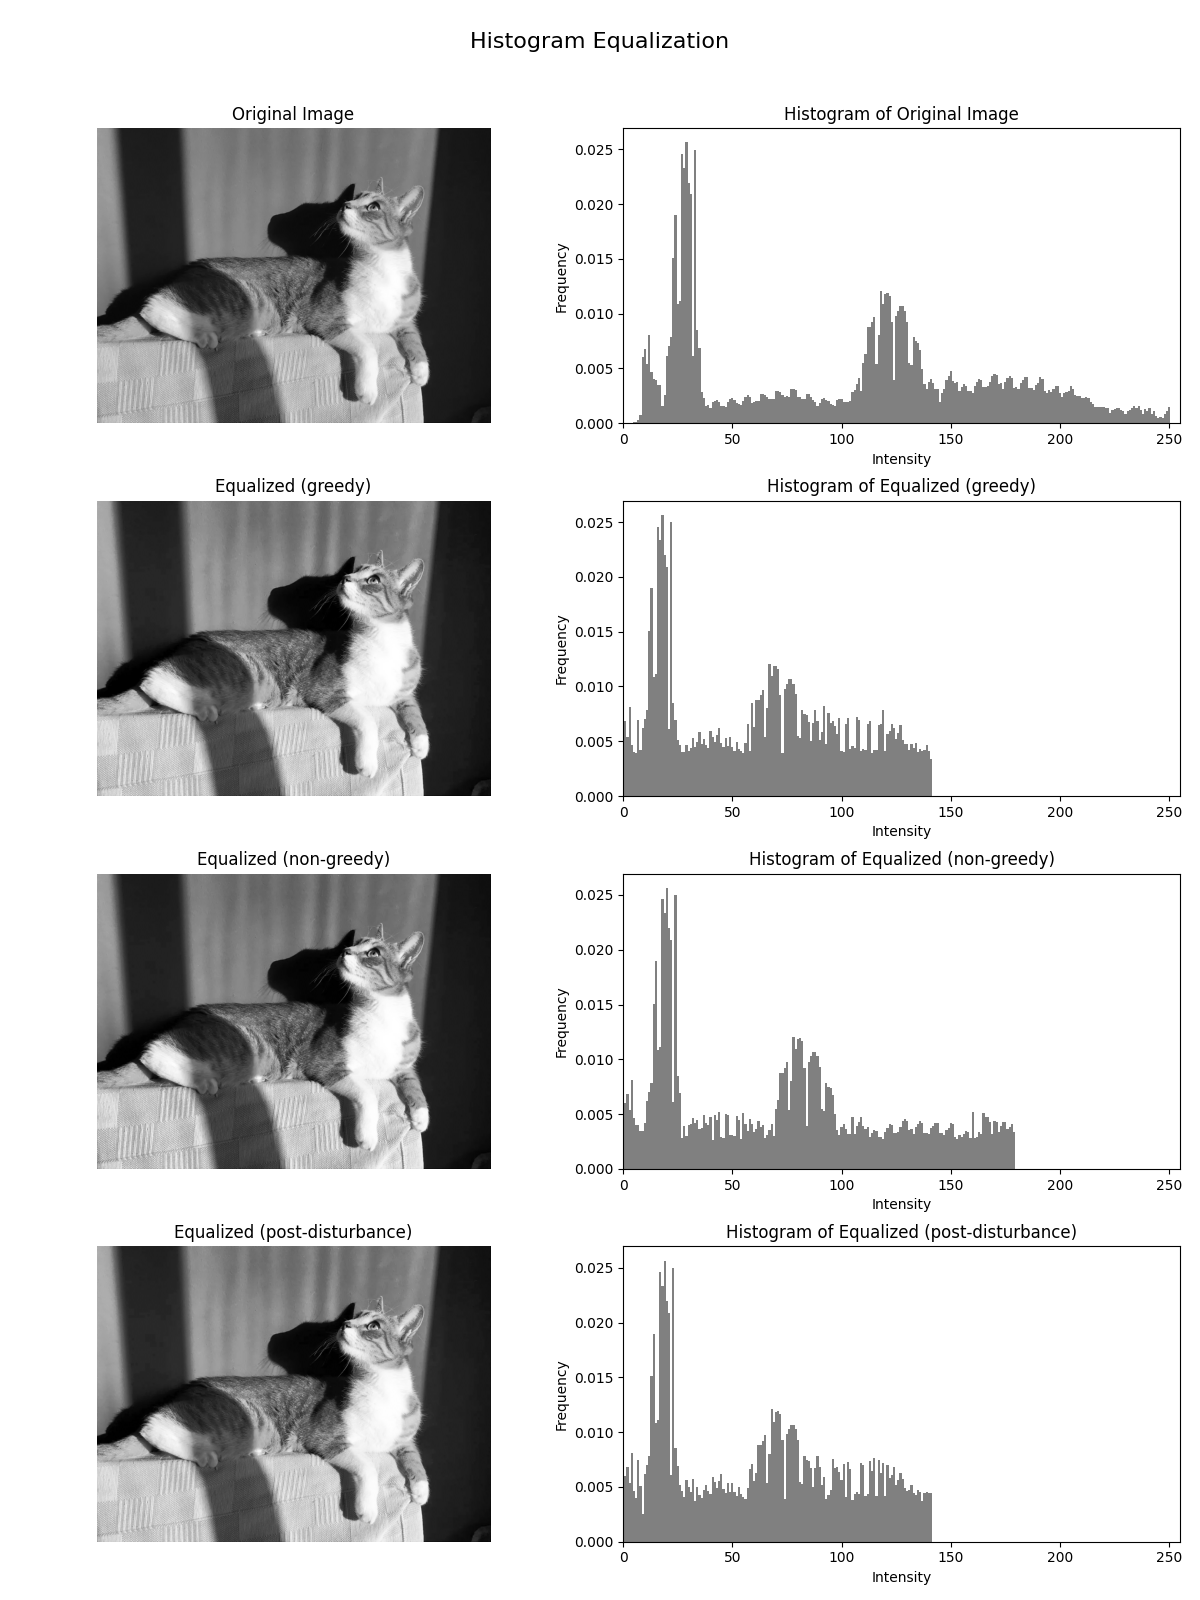
\includegraphics[width=0.8\textwidth]{histogram_equalization_results.png}
  \caption{Equalization: greedy, non-greedy, post-disturbance.}
  \label{fig:eq}
\end{figure}

\begin{figure}[H]
  \centering
  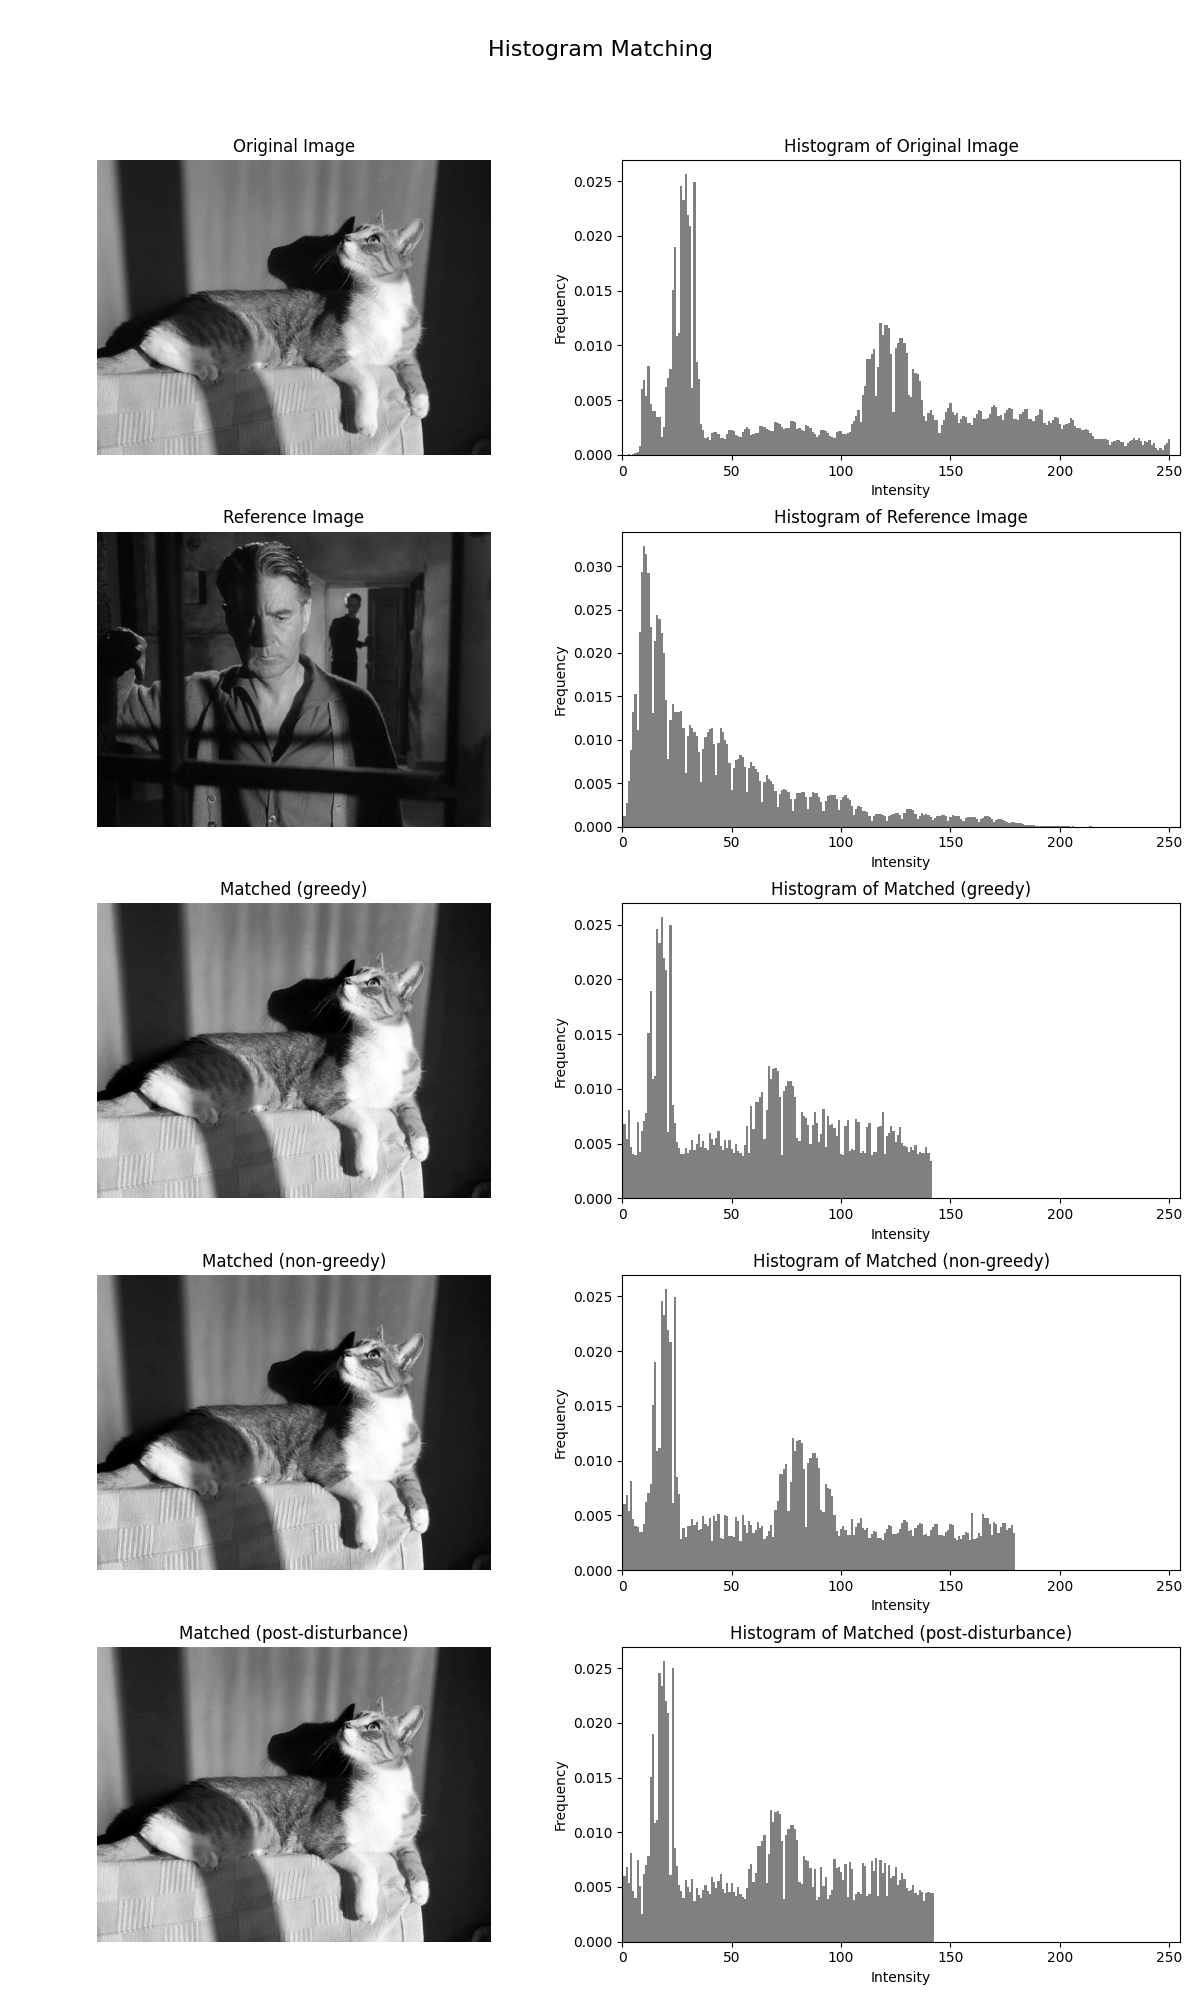
\includegraphics[width=0.8\textwidth]{histogram_matching_results.png}
  \caption{Matching: greedy, non-greedy, post-disturbance.}
  \label{fig:match}
\end{figure}

Όπως διαπιστώνουμε από τα αποτελέσματα οι αλγόριθμοι αντιμετωπίζουν προβλήματα:
\begin{itemize}
  \item \textbf{Αξιοποίηση πλήρους φάσματος}: Σε ιστογράμματα που παρουσιάζουν κυρτότητα ή έχουν πολλές τιμές pixel/δείγματα συγκεντρομένες σε μία/λίγες συχνότητες ο greedy αλγόριθμος αδυνατεί να χρησιμοποιήσει το πλήρες εύρος και να πετύχει καλή εξισορρόπηση ιστογράμματος
  \item \textbf{Non-greedy}: Η non-greedy εκδοχή του αλγορίθμου βελτιώνει την κατανομή αλλά δεν διασφαλίζει και πάλι πλήρες εύρος. Ούτε σε αυτήν την περίπτωση η εξισορρόπηση είναι καλή.
  \item \textbf{Post-disturbance}: Ο αλγόριθμος που χρησιμοποιεί θόρυβο περιορισμένης έκτασης από ομοιόμορφη κατανομή δεν καταφέρνει να επεκτείνει
  αρκετά τις απομακρυσμένες τιμές ώστε να λύσει το πρόβλημα της greedy εκδοχής και έχει παρόμοια αποτελέσματα.
  \item \textbf{Reference Matching}: Παρόμοια αποτελέσματα διαπιστώνουμε και στην περίπτωση της αντιστοίχισης ιστογράμματος σε μία εικόνα αναφοράς. 
\end{itemize}

\section{Επιπρόσθετα Αποτελέσματα}
\begin{figure}[H]
  \centering
  \includegraphics[width=0.8\textwidth]{histogram_equalization_results2.png}
  \caption{Equalization: greedy, non-greedy, post-disturbance.}
  \label{fig:eq}
\end{figure}

\begin{figure}[H]
  \centering
  \includegraphics[width=0.8\textwidth]{histogram_matching_results2.png}
  \caption{Matching: greedy, non-greedy, post-disturbance.}
  \label{fig:match}
\end{figure}

\section{Κώδικας}
Μπορείτε να βρείτε τον κώδικα και τα αποτελέσματα στο \href{https://github.com/charisvt/dip-hw1}{Github}.
\end{document}